\documentclass{article}
\usepackage{graphicx}
\usepackage[hidelinks]{hyperref}
\usepackage[portuguese]{babel}
\usepackage{float}

\title{UAlgeddit}
\author{Desenvolvimento de aplicações para a web \\ Martim Neves, a86010}
\date{\today}

\begin{document}
	\maketitle
	
	\tableofcontents
	
	\newpage
	
	\section{Introdução}
	Desenvolveu-se uma aplicação web com o intuito de facilitar a partilha de informação e interação entre indivíduos.\\
	A aplicação denomina-se "UAlgeddit" e como o nome indica é uma aplicação semelhante ao Reddit.
	
	
	\section{Backend}
	O backend inclui a API e a base de dados utilizados para tornar a aplicação uma realidade.
		
	\subsection{Funcionalidades}
	Através de HTTP requests é possível efetuar as seguintes operações:
	\begin{itemize}
		\item Efetuar login, recebendo um Json Web Token para manter o estado de autenticação.
		\item Efetuar registo de modo a criar conta na aplicação.
		\item Fazer logout, removendo o token do local storage e dando-lhe blacklist.
		\item É possível obter informações acerca de um utilizador.
		\item Um utilizador pode atualizar o seu perfil.
		\item É possível transmitir mensagens em tempo real a partir de uma websocket.
		\item É possível criar subgeddits (versão dos subreddits). O seu criador pode editá-los e removê-los também. Também é possível listar todos os subgeddits e obter detalhes acerca dos mesmos. Todas as operações CRUD estão disponíveis para esta entidade.
		\item É possível criar posts e o seu dono pode eliminá-los também. É também possível dar upvote ("like") ou downvote ("dislike") para além disso também dá para listar e obter detalhes acerca dos posts.
		\item É possível criar comentários e os comentadores podem eliminar os seus comentários. É possível listar todos os comentários para um determinado post.
		\item É possível enviar pedidos de amizade, listar os pedidos de amizade recebidos, aceitar e recusar pedidos de amizade. É também possível desfazer a amizade.
	\end{itemize}
	\subsection{Requisitos}
	Os requisitos tratam-se das funcionalidades, qualidades e restrições contratuais as quais a aplicação tem de cumprir.
	\subsubsection{Requisitos Funcionais}
		Os requisitos funcionais indicam todas as funcionalidades associadas ao backend da aplicação.
		\begin{table}[H]
			\centering
			\begin{tabular}{|c|p{14cm}|}
				\hline
				ID & Descrição \\
				\hline
				RF-01 & O utilizador pode registar-se na plataforma \\
				\hline
				RF-02 & O utilizador pode autenticar-se na plataforma \\
				\hline
				RF-03 & Aquando de um registo na plataforma é automaticamente criado um perfil para o utilizador \\
				\hline
				RF-04 & O utilizador pode criar um subgeddit. \\
				\hline
				RF-05 & O utilizador pode criar posts num subgeddit \\
				\hline
				RF-06 & O utilizador pode comentar qualquer post \\
				\hline
				RF-07 & O utilizador pode dar upvote nos posts \\
				\hline
				RF-08 & O utilizador pode dar downvote nos posts \\
				\hline
				RF-09 & O utilizador tem acesso a um feed com os posts dos vários subgeddits. \\
				\hline
				RF-10 & O karma de um utilizador é definido de acordo com o número de upvotes e downvotes que recebeu nos seus posts de acordo com a seguinte fórmula: (upvotes - downvotes) \\
				\hline
				RF-11 & O utilizador pode consultar o seu perfil. \\
				\hline
				RF-12 & O utilizador pode editar o seu perfil. \\
				\hline
				RF-13 & O utilizador pode eliminar os seus comentários. \\
				\hline
				RF-14 & O utilizador pode eliminar os seus posts. \\
				\hline
				RF-15 & O utilizador pode eliminar os seus subgeddits. \\
				\hline
				RF-16 & O utilizador pode modificar o seu perfil \\
				\hline
				RF-17 & O utilizador pode modificar os seus subgeddits \\
				\hline
				RF-18 & O utilizador tem acesso a uma lista dos subgeddits. \\
				\hline
				RF-19 & O utilizador pode enviar pedidos de amizade a outros utilizadores \\
				\hline
				RF-20 & O utilizador pode aceitar pedidos de amizade. \\
				\hline
				RF-21 & A aplicação dispõe de um chat global entre todos os utilizadores conectados à aplicação \\
				\hline
			\end{tabular}
			\caption{Requisitos Funcionais}
		\end{table}
		\subsubsection{Restrições}
		As restrições indicam todas as restrições inerentes ao desenvolvimento do backend.
		\begin{table}[H]
			\centering
			\begin{tabular}{|c|p{14cm}|}
				\hline
				ID & Descrição \\
				\hline
				RC-1 & Toda a aplicação tem de ser desenvolvida recorrendo à linguagem de programação Typescript. \\
				\hline
				RC-2 & É imperativa a utilização da framework Express para o desenvolvimento do backend. \\
				\hline
				RC-3 & A API interage com o sistema de gestão de base de dados SQLite. \\
				\hline
				RC-4 & O backend tem de estar pronto antes do dia 20 de dezembro de 2025. \\
				\hline
			\end{tabular}
			\caption{Restrições}
		\end{table}
	\subsection{API}
	A API foi desenvolvida recorrendo à linguagem de programação Typescript e à framework Express. \\
	Segue a especificação dos endpoints da API e uma breve descrição de cada um. \\
	Cada um dos tópicos que se seguem corresponde a um Router implementado em Express. \\
	Todos os endpoints excepto o de login e registo estão protegidos por um middleware que verifica se o utilizador está autenticado e apenas deixa utilizadores autenticados aceder a esses mesmos endpoints. \\
	É possível interagir com a API através de http requests. \\
	\subsubsection{Auth}
	
	\begin{itemize}
		\item \textit{POST /auth/login}: Permite autenticar um utilizador.
		\item \textit{POST /auth/register}: Permite registar um utilizador.
		\item \textit{POST /auth/logout}: Efetua o logout de um utilizador.
	\end{itemize}
	
	\subsubsection{Subgeddit}
	
	\begin{itemize}
		\item \textit{POST /subgeddit/create}: Permite criar um subgeddit.
		\item \textit{POST /subgeddit/update/:id}: Permite a partir do id de um subgeddit modificá-lo.
		\item \textit{GET /subgeddit/list}: Lista todos os subgeddits.
		\item \textit{GET /subgeddit/detail/:id}: Permite obter detalhes acerca do subgeddit especificado pelo id.
		\item \textit{POST /subgeddit/delete/:id}: Permite eliminar o subgeddit especificado pelo id.
	\end{itemize}
	
	\subsubsection{Posts}
	
	\begin{itemize}
		\item \textit{POST /post/create}: Permite criar um post.
		\item \textit{POST /post/delete/:id}: Permite eliminar o post especificado pelo id.
		\item \textit{GET /post/list}: Lista todos os posts.
		\item \textit{POST /post/detail/:id}: Permite obter detalhes acerca do post especificado pelo id.
		\item \textit{POST /post/upvote/:id}: Permite dar upvote ao post especificado pelo id.
		\item \textit{POST /post/downvote/:id}: Permite dar downvote ao post especificado pelo id.
		\item \textit{POST /post/unvote/:id}: Permite remover o voto (downvote ou upvote) do post especificado pelo id.
	\end{itemize}
	
	\subsubsection{Comments}
	
	\begin{itemize}
		\item \textit{POST /comment/create}: Permite criar um comentário.
		\item \textit{POST /comment/delete/:id}: Permite eliminar o comentário especificado pelo id.
		\item \textit{GET /comment/list/:pid}: Lista todos os comentários associados ao post com o id = pid.
	\end{itemize}
	
	
	\subsubsection{Profile}
	\begin{itemize}
		\item \textit{GET /profile/view/:id}: Permite obter os detalhes do perfil do utilizador com o id especificado.
		\item \textit{POST /profile/update/}: Permite modificar os dados do perfil do utilizador.
	\end{itemize}
	
	\subsubsection{Friends}
	\begin{itemize}
		\item \textit{POST /friend/request}: Envia um pedido de amizade para um determinado utilizador.
		\item \textit{GET /friend/list}: Lista todos os pedidos de amizade recebidos.
		\item \textit{POST /friend/request/accept}: Permite o utilizador aceitar um pedido de amizade.
		\item \textit{POST /friend/request/decline}: Permite o utilizador rejeitar um pedido de amizade.
		\item \textit{POST /friend/unfriend}: Permite o utilizador terminar a sua amizade com um utilizador em específico.
	\end{itemize}
	
	\subsubsection{Chat}
	\begin{itemize}
		\item \textit{WS /chat/global}: Este é um endpoint especial que disponibiliza uma websocket de modo a tornar possível a comunicação em tempo real entre todos os utilizadores conectados ao chat.
	\end{itemize}
	\subsection{Base De Dados}
	De modo a desenvolver uma base de dados seguindo as melhores práticas desenvolveu-se um modelo relacional e entidade relação de modo a ilustrar as relações entre as entidades e facilitar o desenvolvimento das queries.
	Para além de queries também foram desenvolvidos alguns triggers de modo a facilitar certas queries.
	O sistema de gestão de base de dados utilizado no desenvolvimento da aplicação foi SQLite.
	\subsubsection{Modelo Entidade Associação}
	\begin{figure}[H]
		\centering
		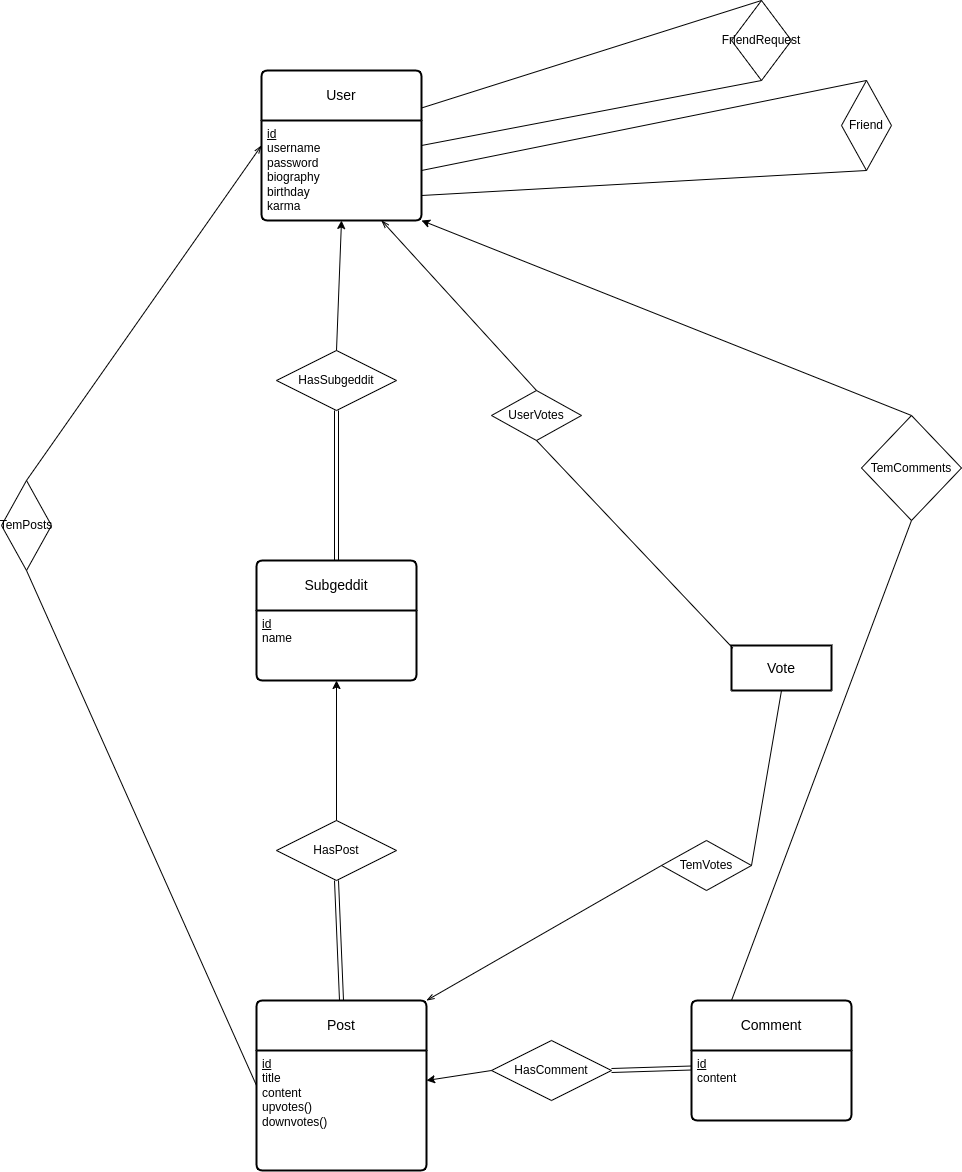
\includegraphics[width=1\textwidth]{ERBD.png}
		\caption{Modelo Entidade Associação}
	\end{figure}
	
	\subsection{Modelo Relacional}
	
	User(id, username, password, karma, biography, birthday)\\
	NN(username)\\
	NN(password)\\
	NN(karma)\\
	RI: O karma tem de ser maior ou igual zero.\\
	RI: O birthday tem de ser antes da data atual.\\
	\\
	Subgeddit(id, name, user\_id)\\
	FK(user\_id) → User\\
	NN(name)\\
	NN(user\_id)\\
	\\
	Post(id, title, content, subgeddit\_id, user\_id)\\
	FK(subgeddit) → Subgeddit\\
	FK(user\_id) → User\\
	NN(title)\\
	NN(content)\\
	NN(subgeddit\_id)\\
	NN(user\_id)\\
	\\
	Comment(id, content, post\_id, user\_id)\\
	NN(content)\\
	NN(post\_id)\\
	NN(user\_id)\\
	FK(post\_id) → Post\\
	FK(user\_id) → User\\
	\\
	FriendRequest(from, to)\\
	FK(from) → User\\
	FK(to) → User\\
	\\
	Friend(user\_id, friend\_id)\\
	FK(user\_id) → User\\
	FK(friend\_id) → User\\
	\\
	Vote(post\_id, user\_id, num)\\
	FK(user\_id) → User\\
	NN(num)\\
	RI: num só pode ser -1 (downvote) ou 1 (upvote)\\

	\section{Frontend}
	
	\subsection{Funcionalidades}
	Ao navegar o Frontend é possível:
	\begin{itemize}
		\item 
	\end{itemize}
	\subsection{Requisitos}
	
	\subsubsection{Requisitos Funcionais}
	
	\subsubsection{Restrições}
	
	\subsubsection{Requisitos de Qualidade}
	
	\subsection{Layout}
	
	\subsection{Set up}
	
	\subsection{Funcionalidades Extra}
	
	\subsubsection{Chat Global}
	
	\subsubsection{Sistema de amizades}
	
	\subsubsection{Perfil e Karma}
	
	

\end{document}